\documentclass[12pt]{article}
\usepackage{amsmath}
\usepackage{graphicx}
\DeclareGraphicsExtensions{.pdf,.png,.jpg}

\newtheorem{theorem}{Theorem}[section]
\newtheorem{lemma}[theorem]{Lemma}
\newtheorem{definition}[theorem]{Definition}


\title{On Sampling}
\date{}
\begin{document}
  \maketitle
  
  \section{Continuous Sampling}
  Consider sampling in a 1D real line $L$. Let $S_{c} = \{q_{x} | \forall x \in L\}$, where $q_{x}$ is a sphere centered at $x$. Let $C(S_{c})$ be the space covered by $S_{c}$.
  
  \begin{theorem}
  Continuously sample spheres from left to right in the real line $L$, let the set of sphere be $S_{n}$, such that no sphere in $S_{n}$ is centered within any sphere of $S_{n}$. Then $C(S_{n}) = C(S_{c})$.
  \end{theorem}
  
  Proof:\\
  
  $\forall x \in L, \exists q_{x} \in S_{c}$, meaning every point in L is covered by one sphere centered at $x$ in $S_{c}$, $C(S_{c}) = L$. If sphere $q_{p}$ is not centered inside any spheres in $S_{n}$, then $q_{p} \in S_{n}$ and $p \in C(S_{n})$. Assume point $p$ is inside some existing spheres centered to the left of $p$, then $p \in C(S_{n})$, but we don't sample spheres at $p$. 
  
  To sum up, if point $p$ is sampled, then $p \in C(S_{c})$ and $p \in C(S_{n})$, if point $p$ is not sampled, still $p \in C(S_{c})$ and $p \in C(S_{n})$. Therefore, $C(S_{n}) = C(S_{c})$.\\
  
  ---------------------------------------------------------------------- \\
  
  This holds true also for 2D and 3D cases. If a point $p$ is sampled, then $p \in C(S_{n})$, if $p$ is not sampled, that is because it is already inside some existing spheres, so $p \in C(S_{n})$.
  
  Continuously sample points that are not inside any sphere is equivalent to continuously sample on the boundary of existing spheres.
  
  \begin{theorem}
  Continuously sample spheres from left to right in the real line $L$, such that no sphere has radius less than $r_{min}$ and no sphere in $S_{m}$ is centered within any sphere of $S_{n}$. $C(S_{m}) = C(S_{c})$.
  \end{theorem}

  Proof:\\
  
  For point $p$ that is within $r_{min}$ distance away from obstacles, there exist a point $x$ that has clearance larger than $r_{min}$, such that $|p-x| > 0$, then p is covered by $q_{x}$.

  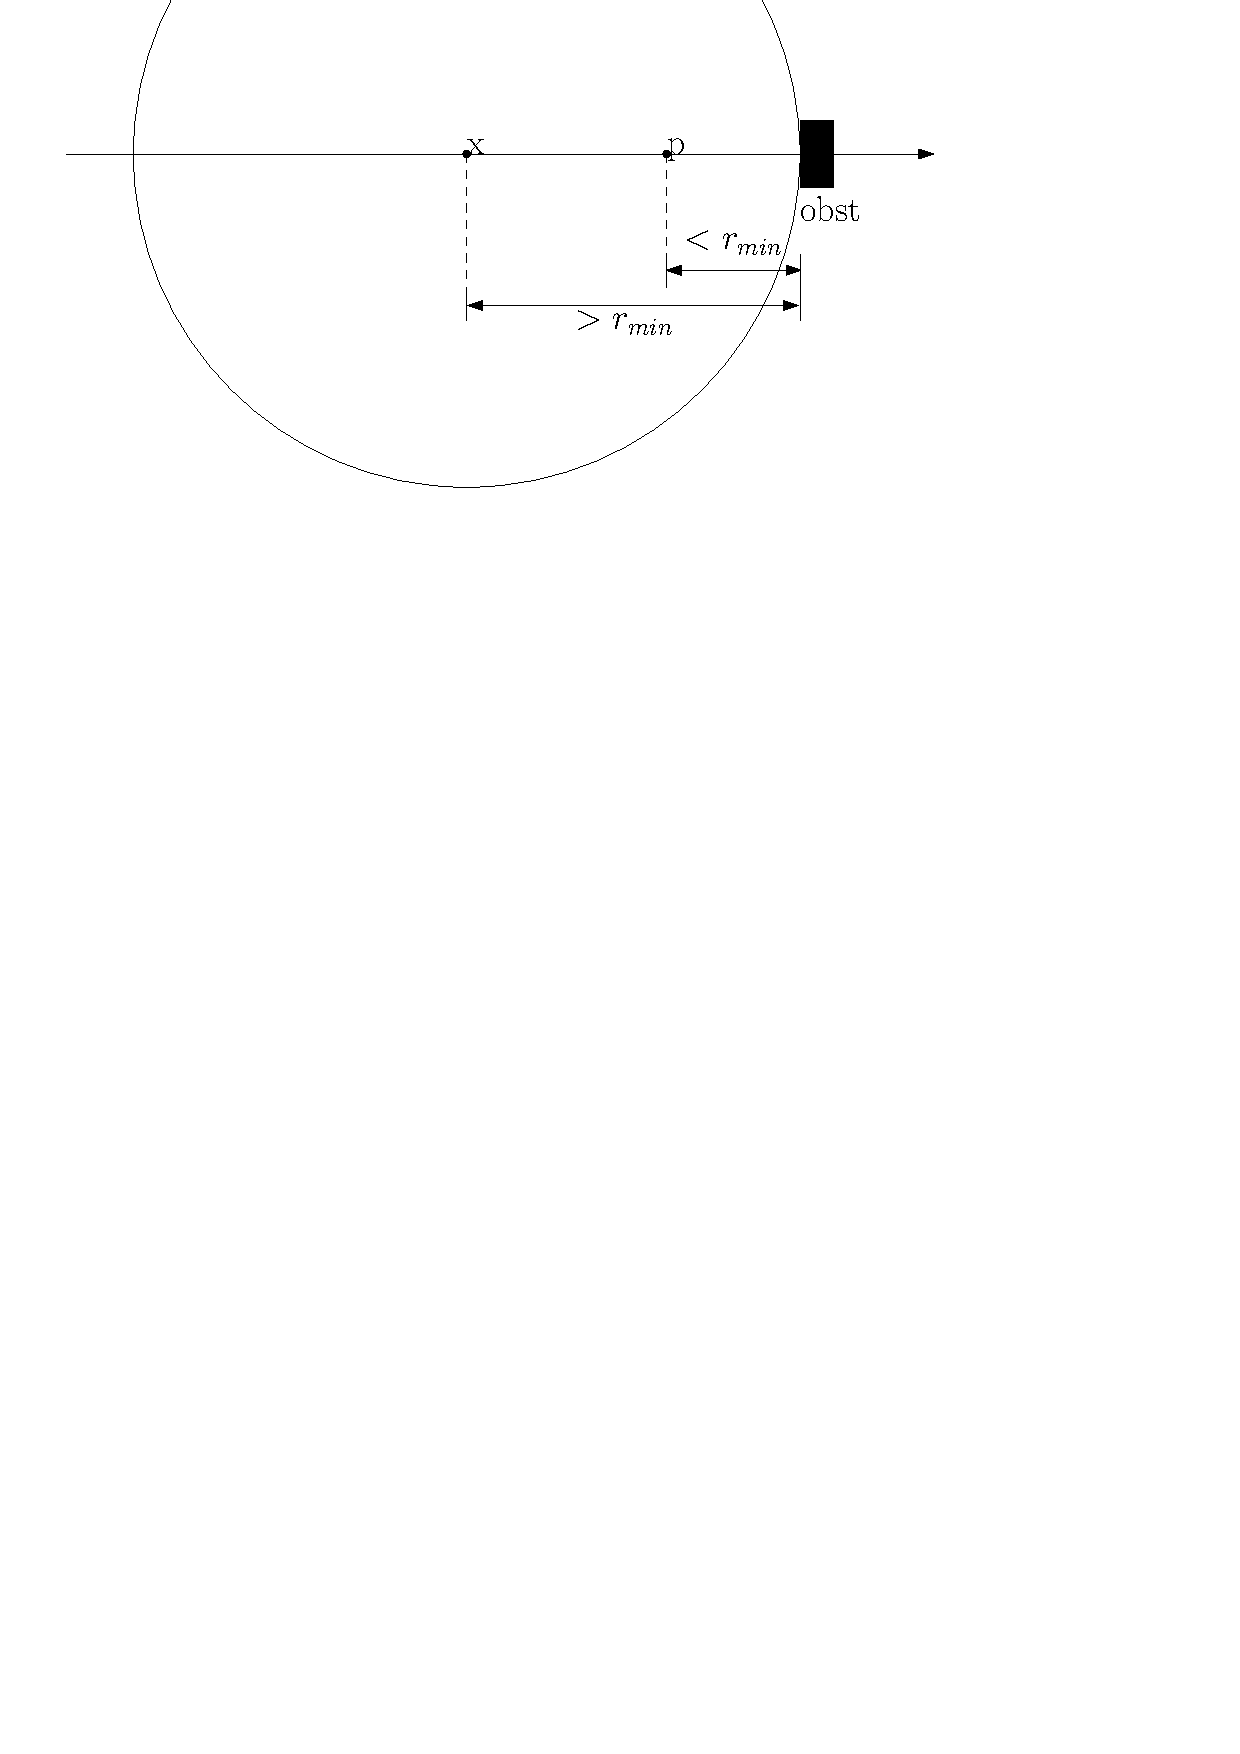
\includegraphics[scale=0.8]{sample_1_2}  
  
  ---------------------------------------------------------------------- \\
  
  For 2D and 3D this is different:\\
  
  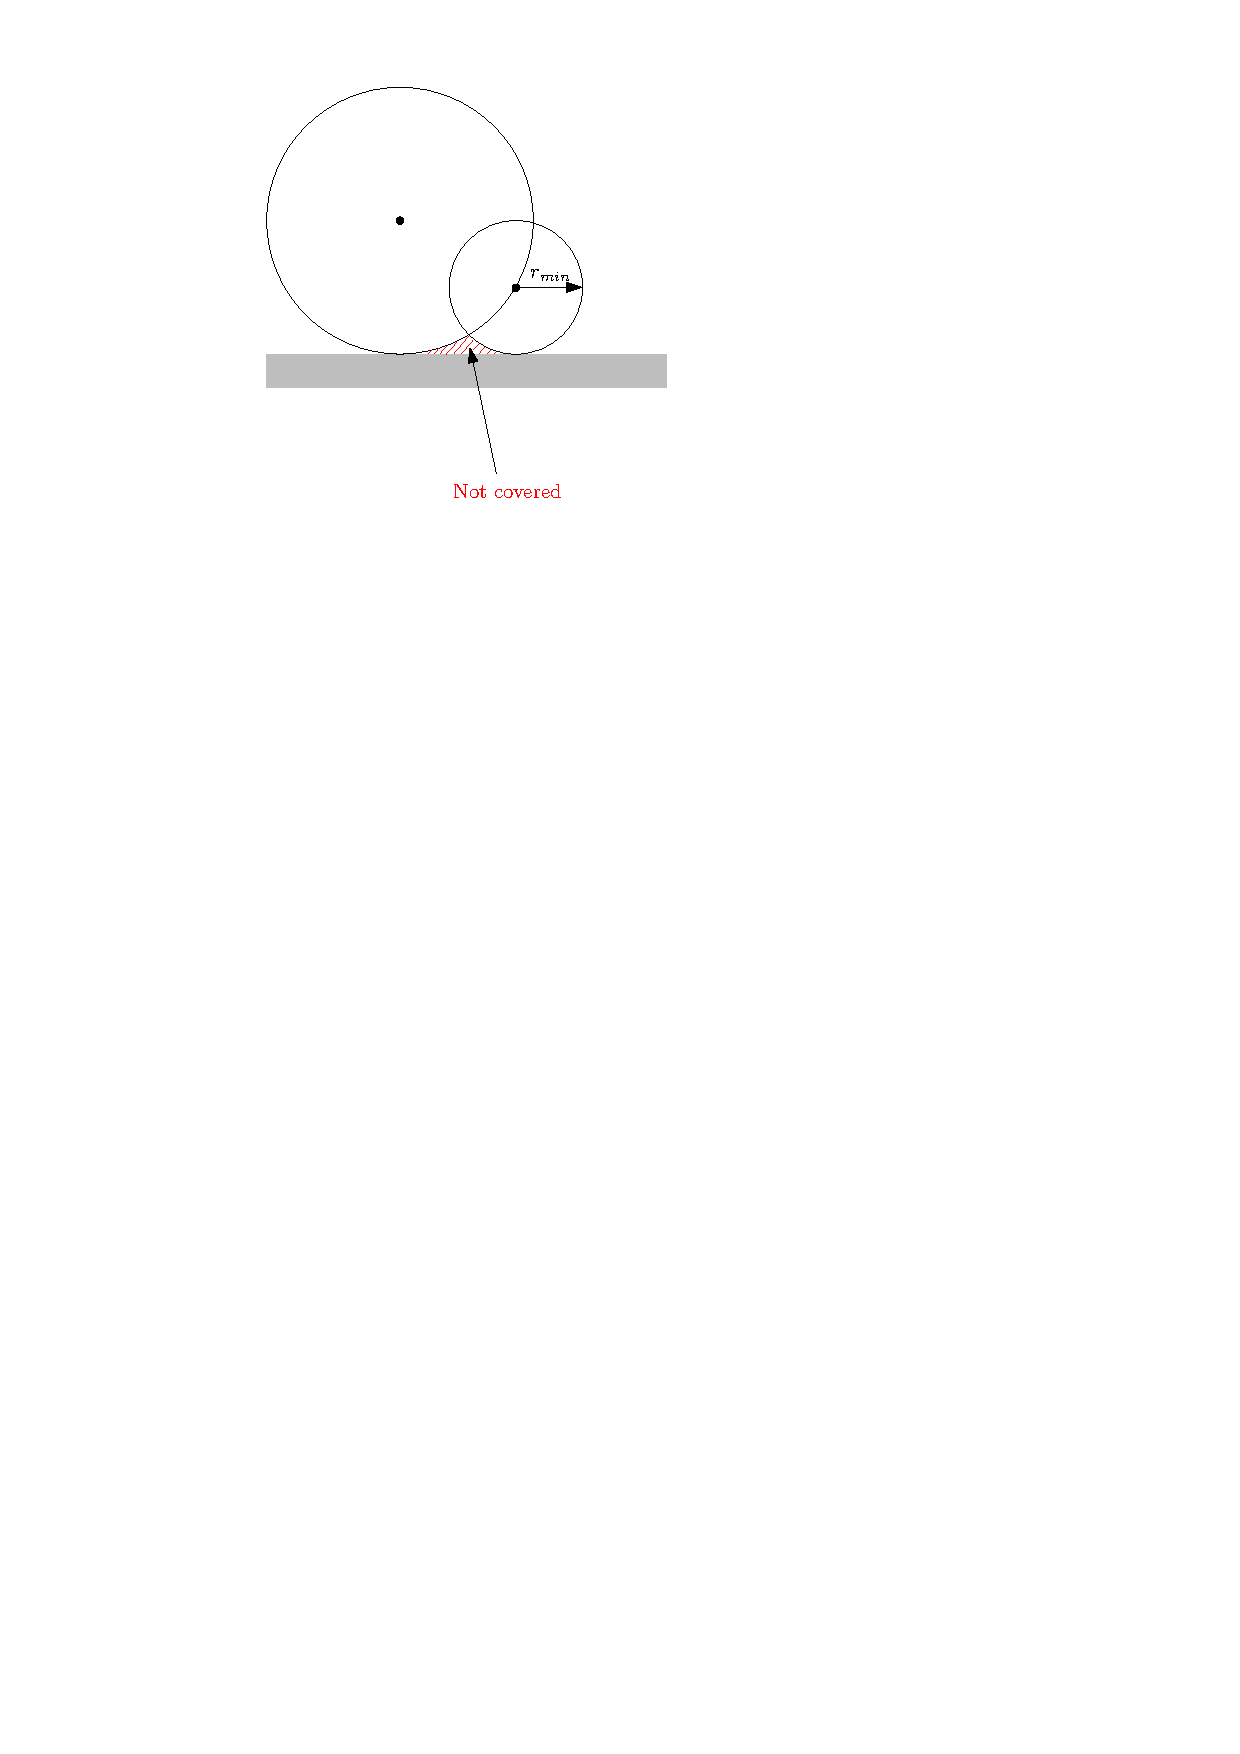
\includegraphics[scale=0.8]{sample2D_1_2}  \\
  
  A possible way to reduce the uncovered area is to more densely sample areas close to obstacles. For example, allow spheres to center inside existing spheres in this area.
  
  
  \begin{theorem}
  Let $S_{in}$ be a subset of $S_{m}$ by continuously sampling spheres from left to right in the real line $L$ with inaccurate metric. Assume the metric returns 1/n of the accurate metric, then any point $p$ within $(n-1) \cdot r_{min}$ distance away from obstacles, $p \notin C(S_(in))$.
  \end{theorem}
  
  Proof:\\
  
  Assume $p$ is $(n-1) \cdot r_{min}$ distance away from obstacles, if there exists point $x$ that is $n \cdot r_{min}$ distance away from obstacles, then sphere $q_{x}$ has radius $r_{min}$, $p \in q_{x}$. 
  
  If $p$ is $(n-1) \cdot r_{min} - \epsilon$ distance away from obstacles, where $\epsilon >= 0$, we need a point $x$ that is within $n \cdot r_{min} - \frac{n \cdot \epsilon}{n-1}$ distance from obstacle.  The sphere sampled at $x$ has radius less than $r_{min}$ thus will not cover point p.\\
 
  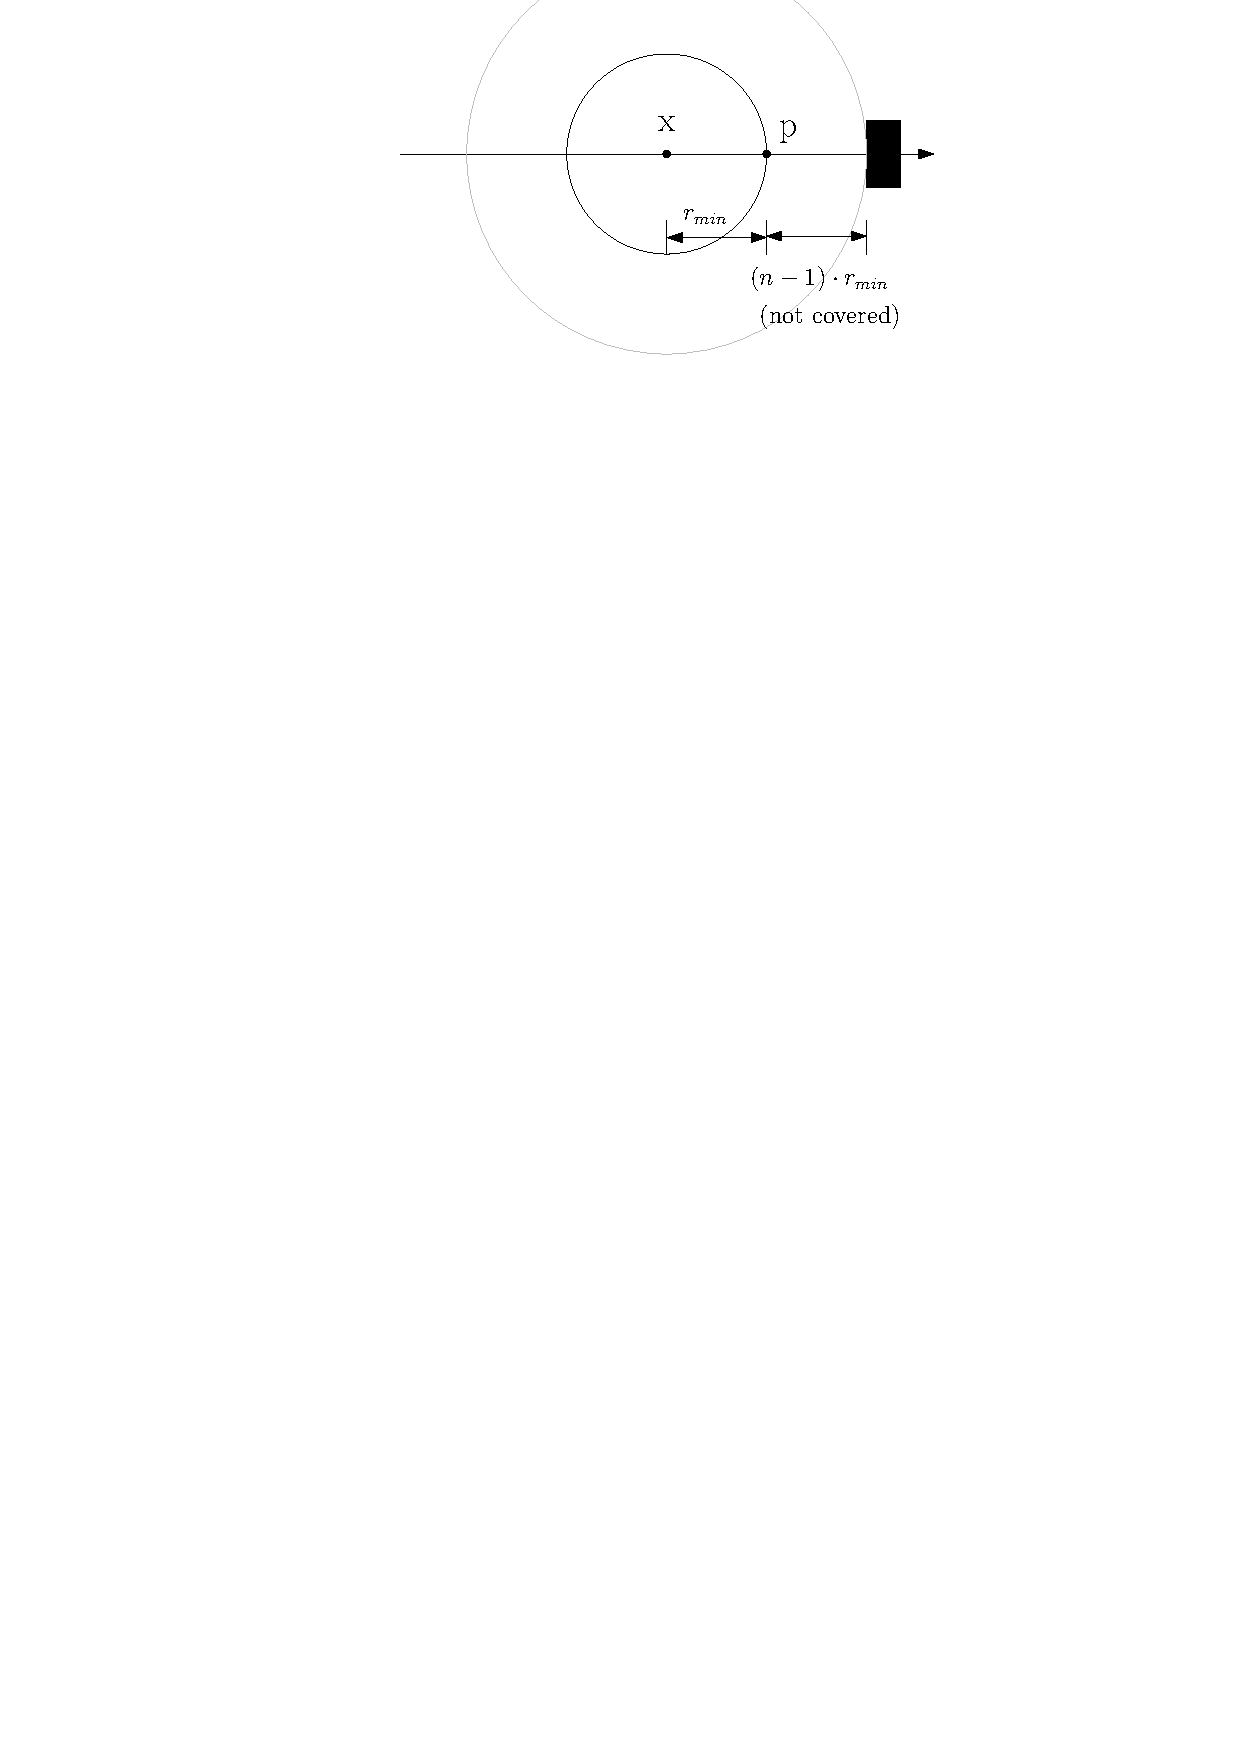
\includegraphics[scale=0.8]{sample_1_3} \\
  
  --------------------------------------------------------------------\\
  
  This is also true for 2D and 3D cases. Introduce a line from the closest point in obstacle in normal direction, then the proof is the same. However, uncovered area as shown in Theorem 1.2 stays still.
  
  \begin{theorem}
  Let $S_{d}$ be a subset of $S_{in}$ by discrete sampling in the real line. Assume every two neighbor samples are $d$ distance away from each other. If $d <= \frac{r_{min}}{k}, k>=1$, in the worst case, any point $p$ that has clearance less than $\frac{r_{min} \cdot (n-1)}{k \cdot n} + (n-1) \cdot r_{min}$, $p \notin C(S_d)$.
  \end{theorem}
  
  As is shown in last theorem, the smallest clearance a point $x$ should have in order to be sampled is $n \cdot r_{min}$. $\exists \epsilon > 0$, point $x_{t}$ with clearance $n \cdot r_{min} + d - \epsilon$. The point the sphere $q_{x_{t}}$ can cover has clearance more than  $(n-1) \cdot r_{min} + \frac{d \cdot (n-1)}{n} - \frac{(n-1) \cdot \epsilon}{n}$. The worst case is $\epsilon = 0$, so the clearance is $(n-1) \cdot r_{min} + \frac{d \cdot (n-1)}{n} = (n-1) \cdot r_{min} + \frac{r_{min} \cdot (n-1)}{k \cdot n}$
    
  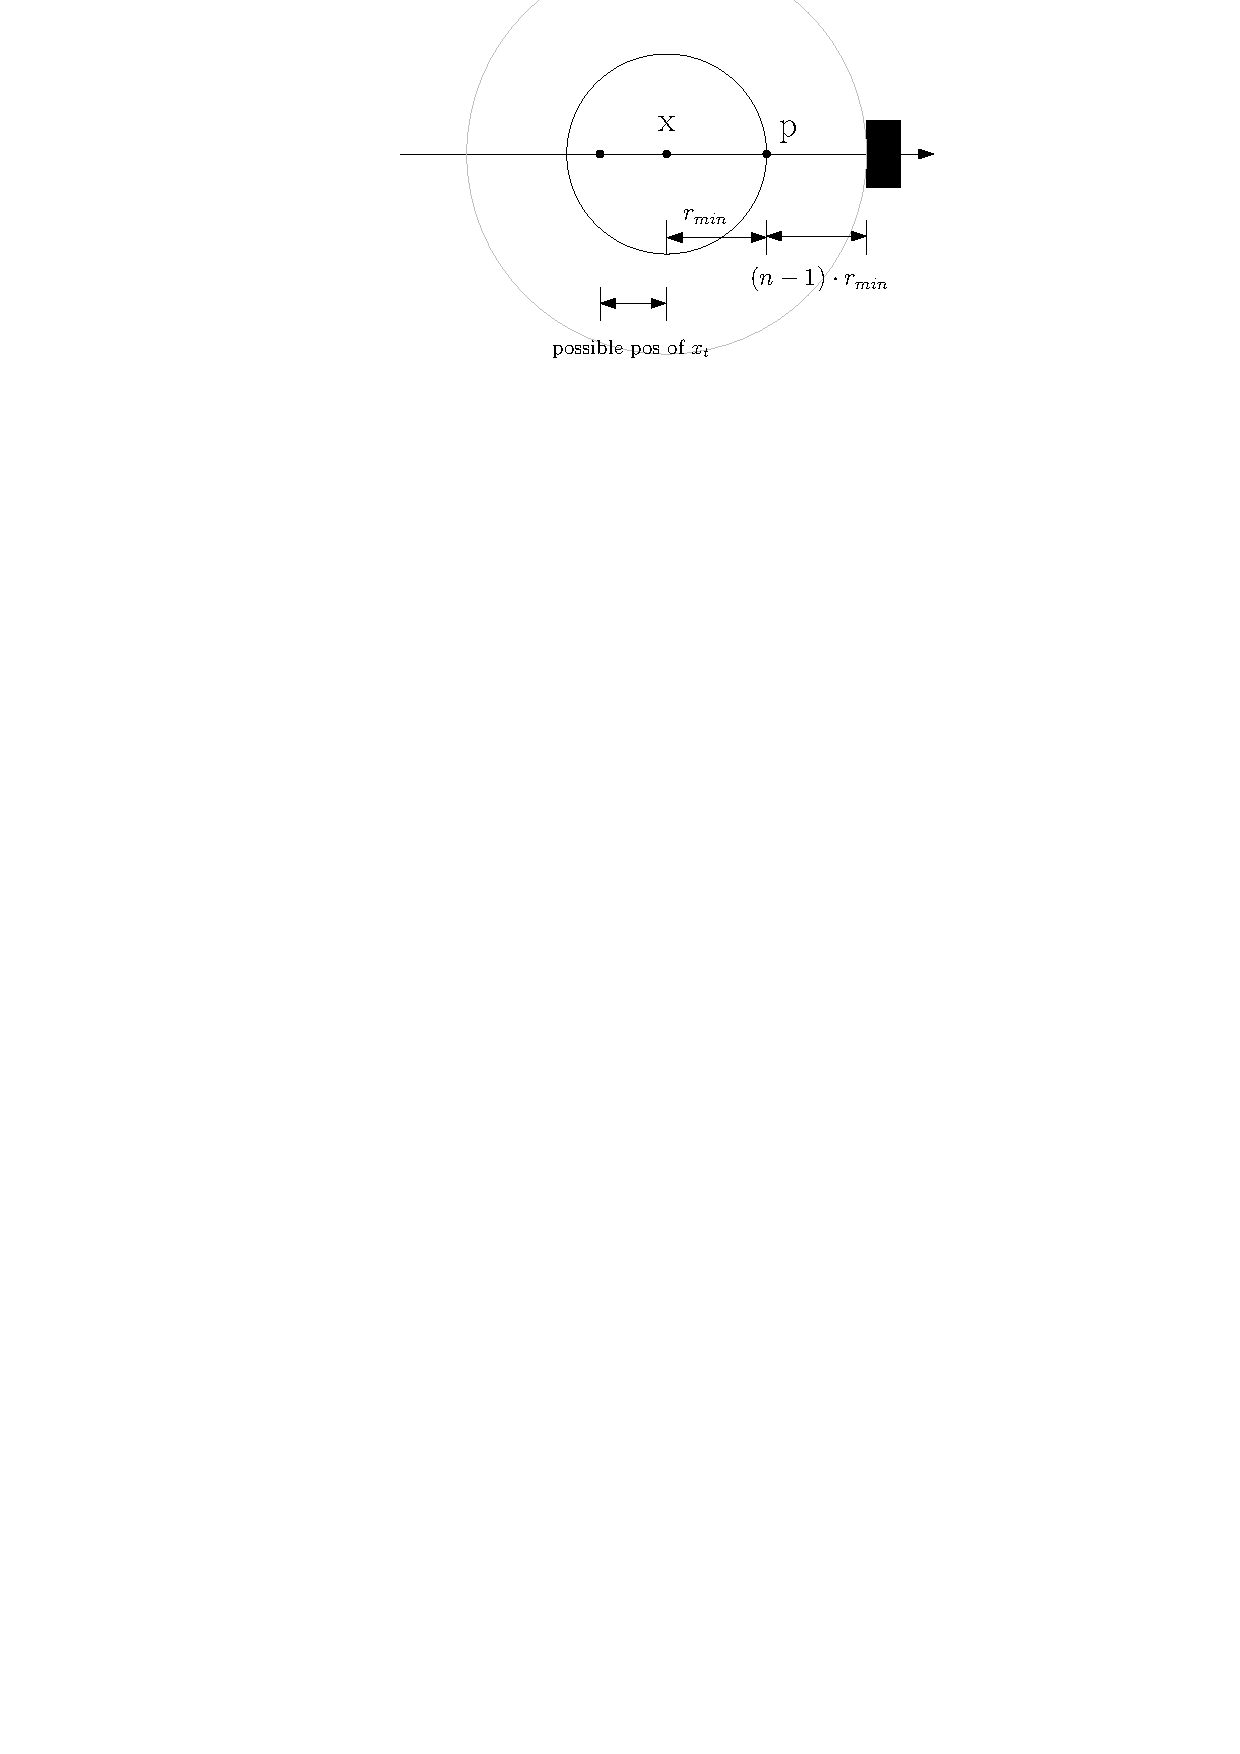
\includegraphics[scale=0.8]{sample_1_4}\\
  
  --------------------------------------------------------------------\\  
  
  In 2D the possible position for $x_{t}$ is a square, it will be a cube in 3D, the result is very similar except for that the uncovered area introduced by Theorem 1.2 is still can't be removed.
  
      
\end{document}
  